\subsection{Collision tests}

With whole blood simulation as the ultimate goal, we must ensure that the method can
effectively capture cell-cell interactions. The RBF-IB method has been applied to flow
around multiple platelets in an aggregate, but those cells are kept apart by a network
of springs~\cite{Shankar:2015km}. To study the interaction between cells, we devise a
series of tests in which we force two RBCs to collide. The aim is to verify that the
cells remain distinct. Using too few data sites could allow the cells to come too close
to one another. The regularization of $\Dirac_h$ then causes them to be treated as a
single unit. Cells that ``fuse'' in this manner are problematic, generally causing the
simulation to end when the cells attempt to separate.

\begin{figure}[t]
    \centering
    \begin{subfigure}[t]{.25\textwidth}
        \centering
        \topinset{(a)}{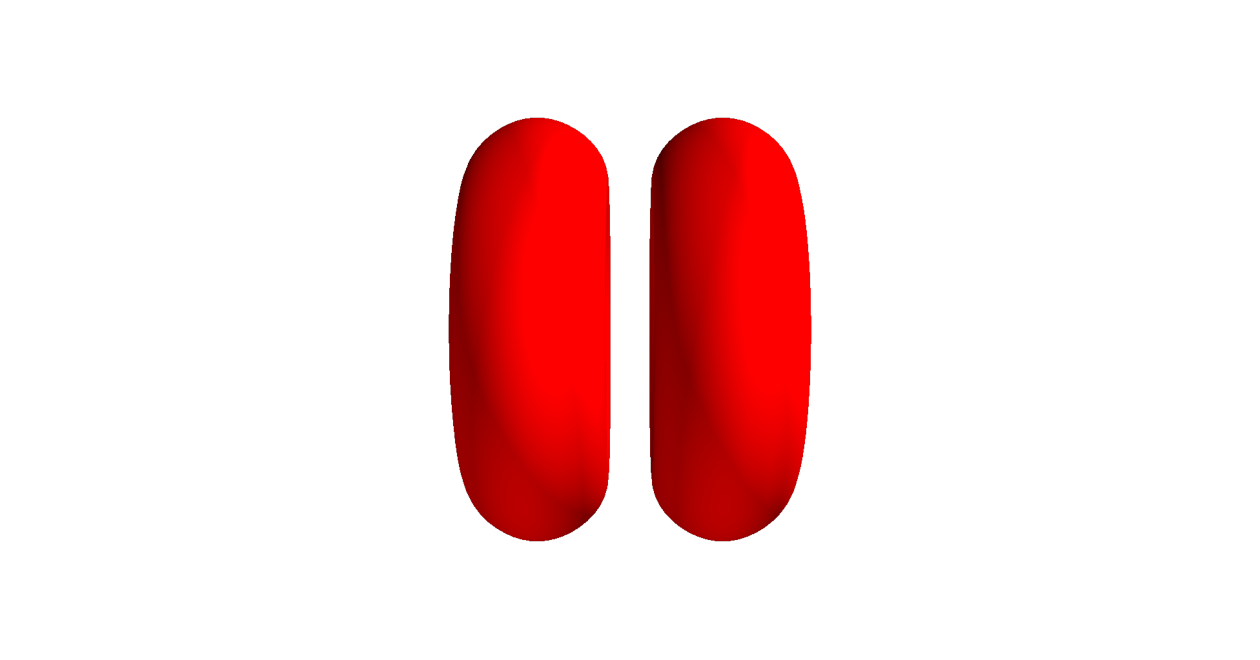
\includegraphics[width=\textwidth]{figures/vvcoll-start.png}}{0.125cm}{0.25cm} \\
        $t = 0\ms$
    \end{subfigure}%
    \begin{subfigure}[t]{.25\textwidth}
        \centering
        \topinset{(b)}{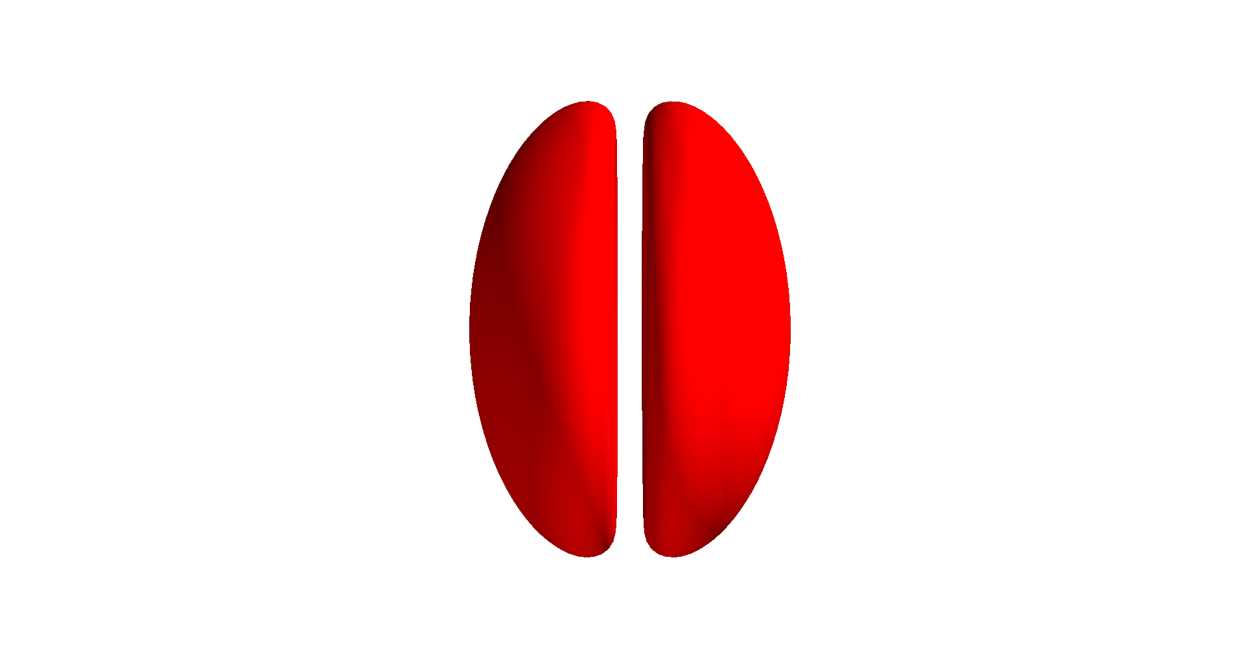
\includegraphics[width=\textwidth]{figures/vvcoll-end.png}}{0.125cm}{0.25cm} \\
        $t = 1.5\ms$
    \end{subfigure}%
    \begin{subfigure}[t]{.25\textwidth}
        \centering
        \topinset{(c)}{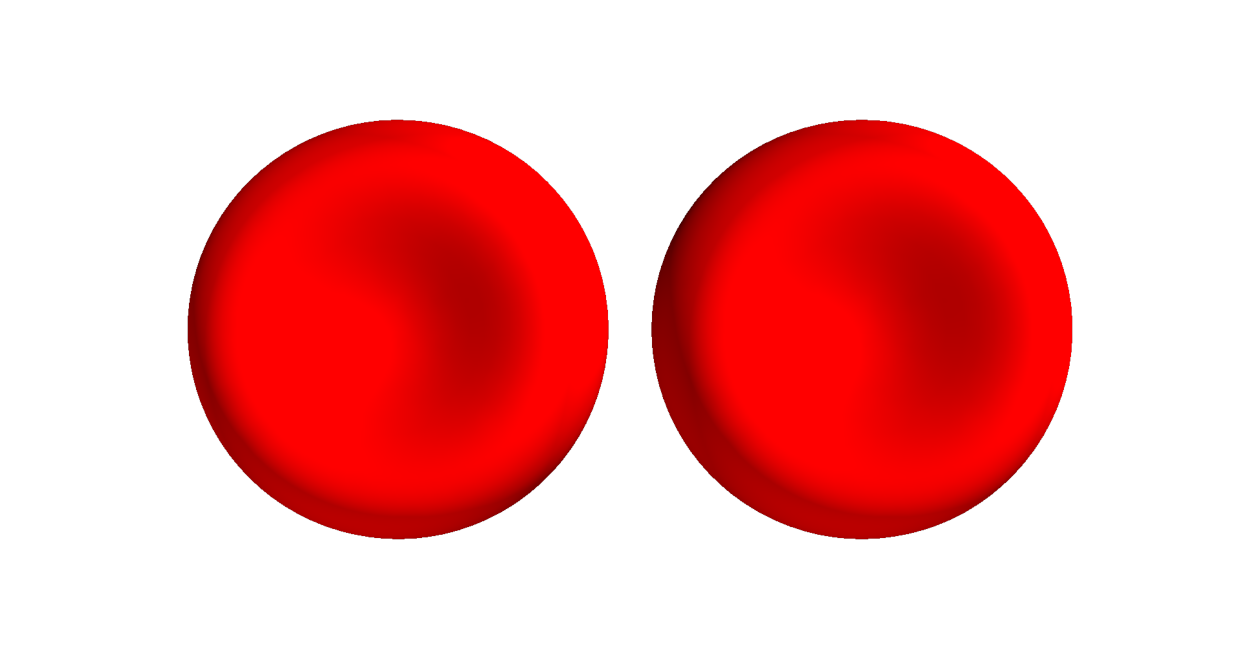
\includegraphics[width=\textwidth]{figures/hhcoll-start.png}}{0.125cm}{0.25cm} \\
        $t = 0\ms$
    \end{subfigure}%
    \begin{subfigure}[t]{.25\textwidth}
        \centering
        \topinset{(d)}{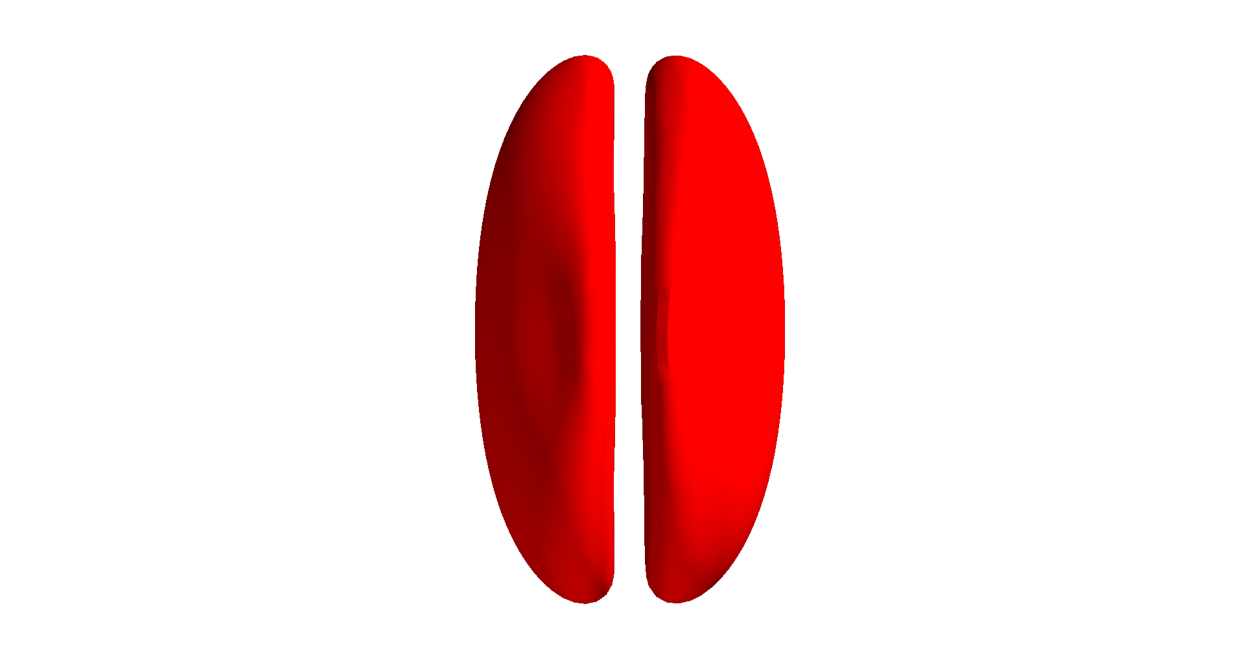
\includegraphics[width=\textwidth]{figures/hhcoll-end.png}}{0.125cm}{0.25cm} \\
        $t = 1.1\ms$
    \end{subfigure}

    \vspace{1em}

    \begin{subfigure}[t]{.25\textwidth}
        \centering
        \topinset{(e)}{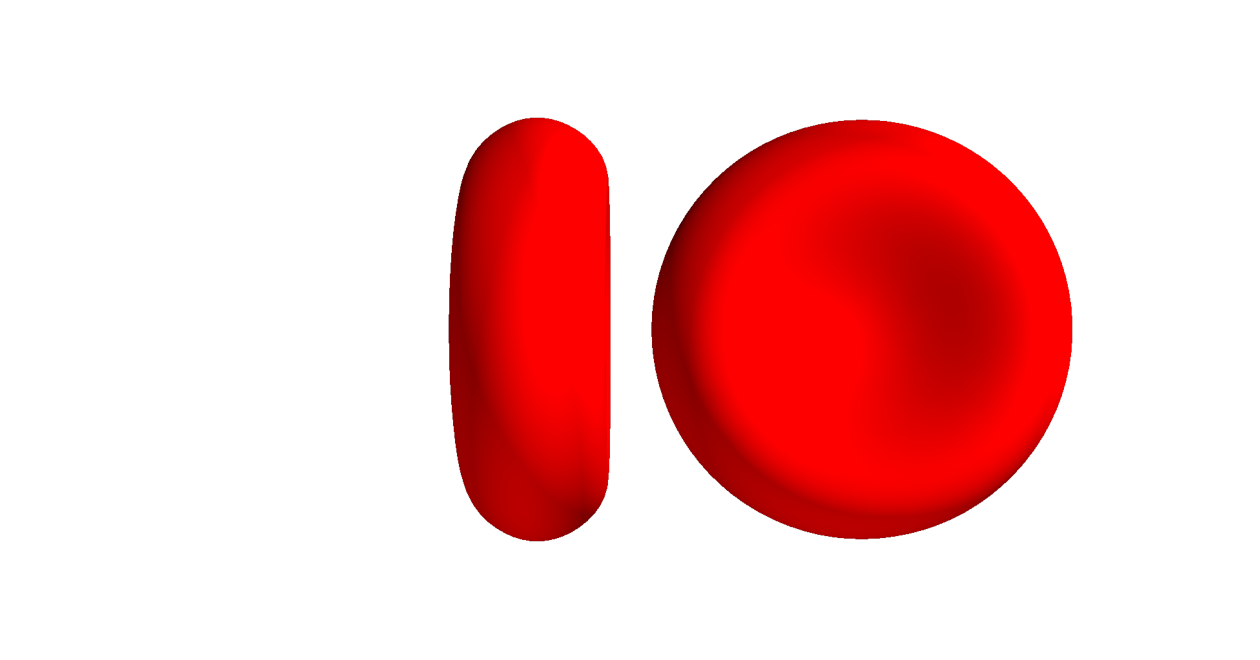
\includegraphics[width=\textwidth]{figures/vhcoll-start.png}}{0.125cm}{0.25cm} \\
        $t = 0\ms$
    \end{subfigure}%
    \begin{subfigure}[t]{.25\textwidth}
        \centering
        \topinset{(f)}{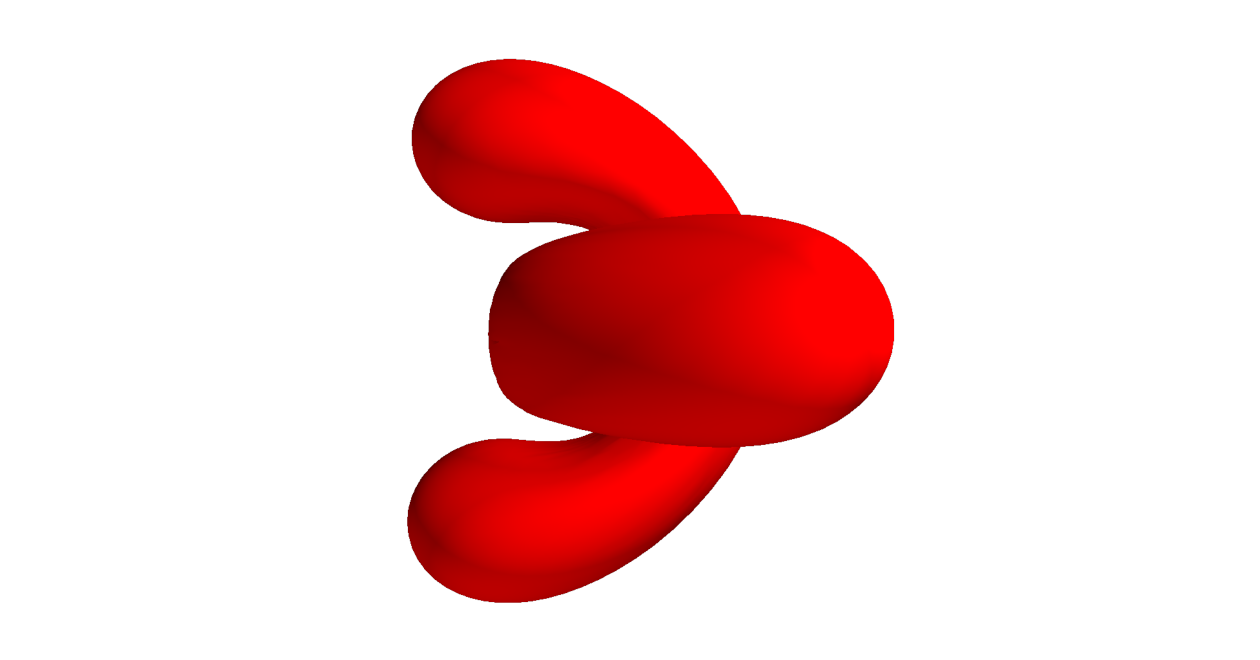
\includegraphics[width=\textwidth]{figures/vhcoll-end.png}}{0.125cm}{0.25cm} \\
        $t = 1.5\ms$
    \end{subfigure}%
    \begin{subfigure}[t]{.25\textwidth}
        \centering
        \topinset{(g)}{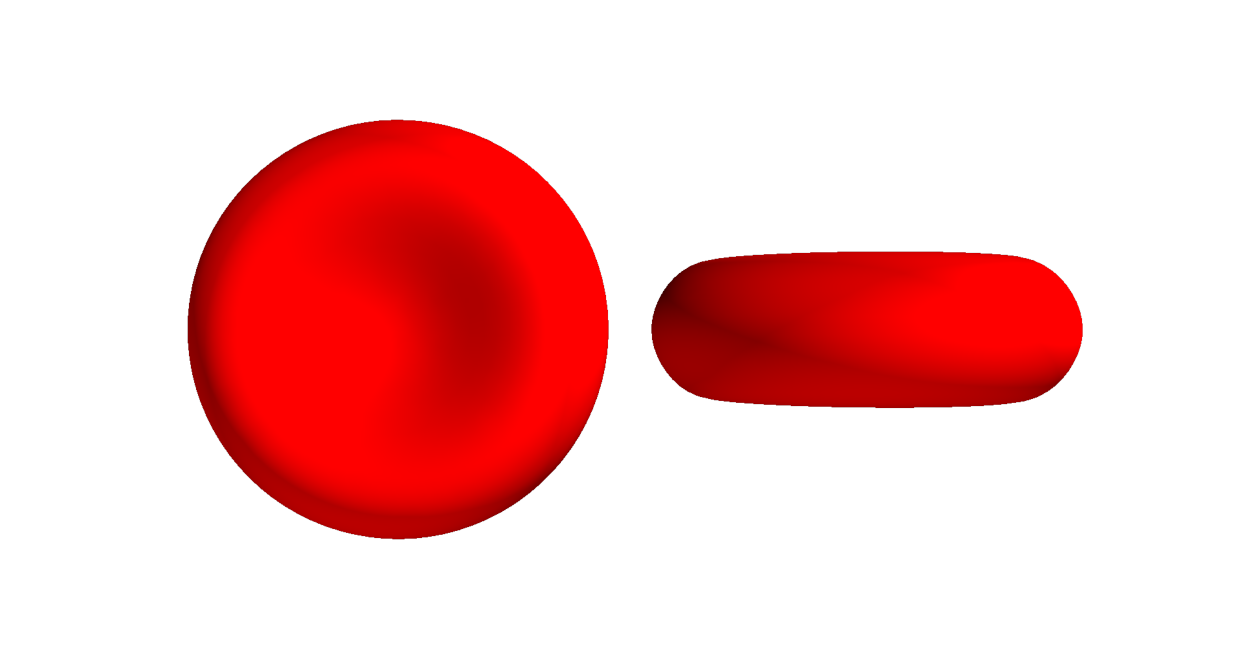
\includegraphics[width=\textwidth]{figures/rhhcoll-start.png}}{0.125cm}{0.25cm} \\
        $t = 0\ms$
    \end{subfigure}%
    \begin{subfigure}[t]{.25\textwidth}
        \centering
        \topinset{(h)}{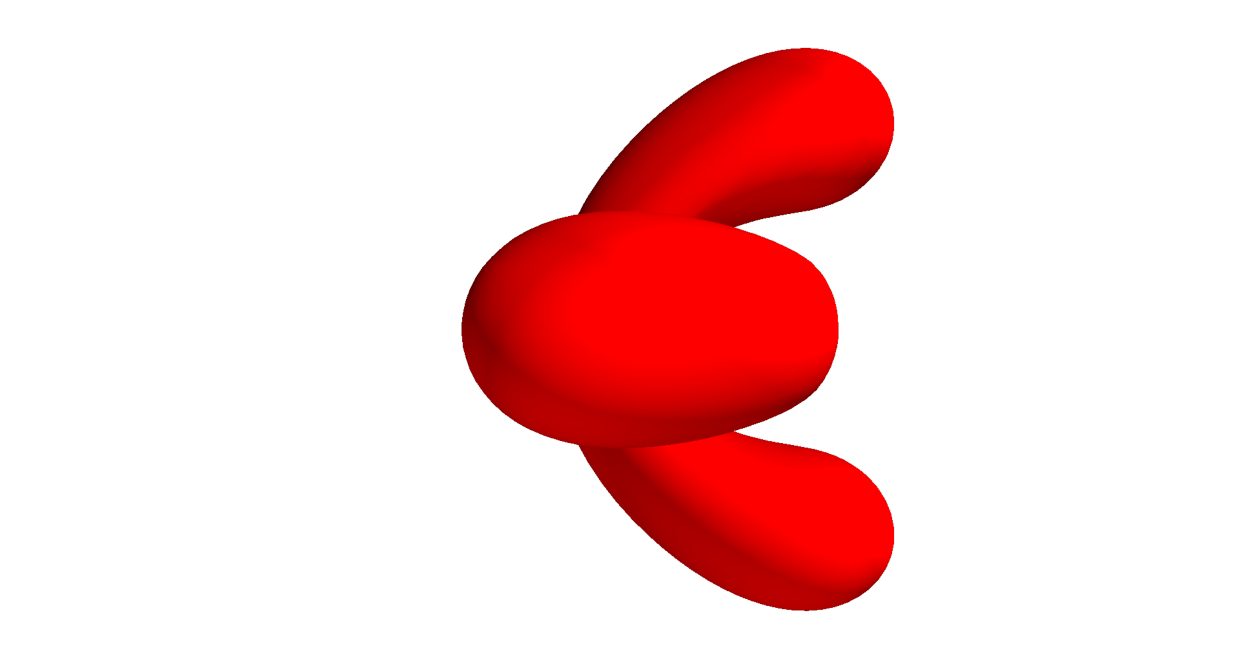
\includegraphics[width=\textwidth]{figures/rhhcoll-end.png}}{0.125cm}{0.25cm} \\
        $t = 1.1\ms$
    \end{subfigure}
    \caption{%
Collision tests between two RBCs. A fictitious force is added to the RBCs to draw them
together. (a--b) The RBCs are initially aligned with concavities facing one another. By
$1.5\ms$, the cells take on a hemispherical shape. The concavities in the gap are
maintained. Shortly thereafter, asymmetries in the setup lead to the cells sliding past
one other. (c--d) The RBCs are initially aligned with their edges facing one
another. By $1.1\ms$, the cells take on a hemispherical shape. The remnants of the
concavity can be seen on the left cell in (d). Shortly thereafter, these cells also slide
past one another. (e--f) The RBCs are initially aligned with the edge of one facing a
concavity of the other. The cells wrap around each other by $1.5\ms$, taking on a bulbous
banana shape. (g--h) The RBCs are initially aligned with their edges facing one another
with one of the cells rotated about the axis $\e_1+\e_3$ by $\pi/2$. By $1.1\ms$, the
cells wrap around each other, again taking on the bulbous banana shape.
    }%
    \label{fig:collisions}
\end{figure}

We continue to use the same physical domain as in the previous two sections, now with
$h = 0.2\um$, and place two RBCs therein, each with $\data\cardinality=2500$ and
$\sample\cardinality=10000$. The ratio $\sample\cardinality/\data\cardinality=4$ is
chosen so that sample sites with spacing $h$ means data sites have spacing $2h$. We
believe this to suffice in preventing cells from intersecting, but this is not guaranteed
if the points do not maintain appropriate spacing throughout a simulation. We use the
2-stage RK method with time step $\timestep = 50\ns$. To interpolate velocities and
spread forces, we use the 4-point cosine $\kernel$~\cite{Peskin:2002go}. The cells are
placed with cell centers on the line $x = z$, $y = 8\um$. They are initially separated by
a gap of $4h = 0.8\um$ between their convex hulls, \latin{i.e.}, ignoring the
concavities. Inspired by Crowl \& Fogelson~\cite{Erickson:2011cf}, we add the fictitious
force density
\begin{equation*}
    \F_\text{fict} = \pm 0.1\dynpercm\cdot(\e_1+\e_3)/\sqrt{2},
\end{equation*}
to each cell, where the sign is chosen so the force points into the gap, to draw the
cells together. Success in these tests implies that this configuration of data and sample
sites, the spatial resolution, and the time step are acceptable for whole blood
simulations.

Initial conditions and configurations after a short time are illustrated in Figure~%
\ref{fig:collisions}, where we view them from above the $x=z$ plane. In each case, the
cells move slightly closer together and then undergo considerable deformation. The data
sites are initially approximately $2h$ apart from each other. No problems seem to arise
from this, and in some cases the cells eventually attempt to slide past one another.  We
also deduce that the IB method with the cosine kernel can resolve interactions at a
distance of $h$ to $2h$. We consider cells passing within this threshold to be in
contact. Throughout the simulation, the cells remain distinct, and the simulations end
due to extreme forces triggering the stopping condition~\cite{Agresar:1998wv}
\begin{equation}
    \timestep > \frac14\sqrt{\frac{h\rho}{\|\f\|_\infty}}.
\end{equation}
For the remainder of this chapter, we will consider only this arrangement of data and
sample sites and this grid resolution.
